\documentclass[11pt]{amsbook}

\usepackage{../HBSuerDemir}

\begin{document}
    \hPage{b1p2/417}

    \begin{center}
        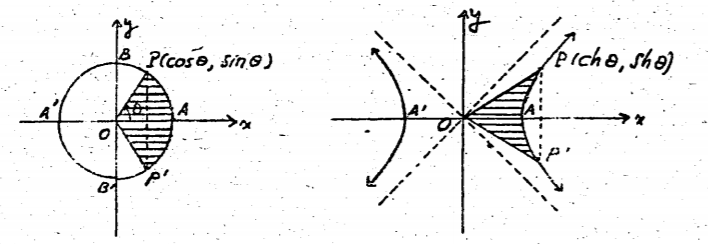
\includegraphics{images/hw1.png}
    \end{center}
    
    We are going to show that $\Theta$ as arc $(angle)$ on the unit
    circle represents the area of the shaded segment of circle bounded by the line segment $(OP),$ $(OP^\prime)$ and the arc $P^\prime AP$, and $\Theta$ as argument in hyperbolic functions represents the area of the shaded region bounded by $(OP),$ $(OP^\prime)$ and the arc of hyperbola $P^\prime AP$.
    
    \begin{hEnumerateAlpha}
        \item $|OP^\prime AP \vert = \frac{2\Theta}{2\Pi} $ $ \Pi r^2 $ $(r = 1) = \Theta$
        \item $|OP^\prime AP \vert = 2 |POH \vert -2|PAH \vert = \operatorname{Ch}\Theta \operatorname{Sh}\Theta - 2 \int_A^P y \,dx$
    \end{hEnumerateAlpha}
    
    $ $\\
    \noindent
    where, having 
    
    \begin{align*}
        2 \int_A^P y \,dx &= 2 \int_0^\Theta \operatorname{Sh}t \,d\operatorname{Ch}t = 2 \int_0^\Theta \operatorname{Sh}t^2 \,dt
        \\
        &= 2 \int_0^\Theta (\operatorname{Ch}2t - 1) \,dt = \frac{1}{2} \operatorname{Sh}2\Theta - \Theta ,
    \end{align*}
    
    \noindent
    we get 
    
    \[
        |OP^\prime AP \vert = \operatorname{Ch}\Theta \operatorname{Sh}\Theta - \frac{1}{2} \operatorname{Sh}2\Theta + \Theta = \Theta
    \]
    
    \section{INVERSE HYPERBOLIC FUNCTIONS.}
    
    Observing from the graphs of hyperbolic functions the all these, except $\operatorname{Ch}x$ and $\operatorname{Sech} x$ are monotone increasing or monotone decreasing on their domain, while\footnote{Since $\operatorname{Ch} x$ ($\operatorname{Sech} x$) is monotone decreasing (increasing) ($-\infty , 0$) also inverse in that interval and the graphs is symmetric of the given one w.r. to x-axis.} $\operatorname{Ch}x$ $\operatorname{Sech} x$

\end{document}